\section*{PHYSIQUE (13 points)}
Exercice 1(2,5 points): Ondes lumineuses\\
La diffraction et la dispersion de la lumière sont deux phénomènes rencontrés dans la vie courante. Ces phénomènes permettent d'expliquer la nature de la lumière, de donner des informations sur les milieux de propagation et de déterminer certaines grandeurs caractéristiques.\\
Donnée: vitesse de propagation de la lumière dans le vide $c=3.10^{8} \mathrm{~m} \cdot \mathrm{~s}^{-1}$.

\begin{enumerate}
  \item Propagation de la lumière à travers un prisme\\
1.1. Une lumière rouge monochromatique, de longueur d'onde dans le vide $\lambda_{0 R}=768 \mathrm{~nm}$, arrive sur un prisme en verre. L'indice du verre pour cette radiation est $n_{R}=1,618$.\\
Pour les deux questions suivantes, recopier sur votre copie le numéro de la question et écrire la lettre correspondante à la proposition vraie parmi:\\
1.1.1. La fréquence $v_{R}$ de la lumière rouge est:
\end{enumerate}

\begin{center}
\begin{tabular}{|l|l|l|l|l|l|l|}
\hline
$\mathbf{a}$ & $v_{R}=2,41.10^{14} \mathrm{~Hz}$ & $\mathbf{b}$ & $v_{R}=3,91.10^{14} \mathrm{~Hz}$ & $\mathbf{c}$ & $v_{R}=2,41.10^{16} \mathrm{~Hz}$ & $\mathbf{d}$ \\
\hline
\end{tabular}
\end{center}

\subsection*{1.1.2. La vitesse $v_{R}$ de propagation de la lumière rouge dans le verre est:}
\begin{center}
\begin{tabular}{|l|l|l|l|l|l|l|}
\hline
$\mathbf{a}$ & $v_{R}=1,20.10^{8} \mathrm{~m}^{-1}$ & $\mathbf{b}$ & $v_{R}=1,55.10^{8} \mathrm{~m}^{-1}$ & $\mathbf{c}$ & $v_{R}=1,85.10^{8} \mathrm{~m} . \mathrm{s}^{-1}$ & $\mathbf{d}$ \\
$v_{R}=1,90.10^{8} \mathrm{~m} . \mathrm{s}^{-1}$ &  &  &  &  &  &  \\
\hline
\end{tabular}
\end{center}

1.2. Lorsqu'une lumière violette monochromatique de longueur d'onde dans le vide $\lambda_{0 V}=434 \mathrm{~nm}$ arrive sur le même prisme, sa vitesse de propagation dans le verre est $v_{V}=1,81.10^{8} \mathrm{~m} . \mathrm{s}^{-1}$.\\
En comparant $v_{R}$ et $v_{V}$, déduire une propriété du verre.

\section*{2. Propagation de la lumière à travers une fente}
On réalise la diffraction de la lumière en utilisant un laser qui donne une lumière monochromatique de longueur d'onde $\lambda$ dans l'air. Cette lumière traverse une fente de largeur $a$ réglable. On obtient une figure de diffraction sur un écran situé à une distance de la fente.\\
On mesure l'écart angulaire $\theta$ pour différentes valeurs a de la largeur de la fente. La courbe ci-contre représente les variations de $\theta$ en fonction de $\left(\frac{1}{a}\right)$.\\
\includegraphics[width=\textwidth]{2025_05_09_728930de905683949ab2g-4(1)}

Recopier sur votre copie le numéro de la question et écrire la lettre correspondante à la proposition vraie parmi:\\
La valeur de la longueur d'onde est:

\begin{center}
\begin{tabular}{|l|l|l|l|l|l|l|l|}
\hline
$\mathbf{a}$ & $\lambda=400 \mathrm{~nm}$ & $\mathbf{b}$ & $\lambda=440 \mathrm{~nm}$ & $\mathbf{c}$ & $\lambda=680 \mathrm{~nm}$ & $\mathbf{d}$ & $\lambda=725 \mathrm{~nm}$ \\
\hline
\end{tabular}
\end{center}

\section*{Exercice 2 (5 points) : Circuit RLC série}
Un ensemble de circuits électriques et électroniques comportent des
condensateurs et des bobines. Le comportement de ces circuits diffère selon
l'effet imposé par ces composants. Le but de cet exercice est d'étudier un
circuit RLC série dans différents cas.

\begin{minipage}{0.70\linewidth}
    On réalise le montage expérimental représenté sur la
    Fig.~\ref{fig:2bac_svt_national_2017_normale_phys_ex2_1} qui comporte~:
    \begin{itemize}
        \item un générateur idéal de tension de force électromotrice
              ${E=\qty{6}{\volt}}$~;
        \item un condensateur de capacité $C$~;
        \item un conducteur ohmique de résistance $R$~;
        \item une bobine $b$ d'inductance $L$ et de résistance $r$~;
        \item un interrupteur $\mathrm{K}$.
    \end{itemize}
\end{minipage}
\hfill
\begin{minipage}{0.28\linewidth}
    \flushright
    \begin{figure}[H]
    \begin{circuitikz}
        \newdimen\d \d=3cm
        \draw (0,0) node[cute spdt mid,rotate=90] (Sw) {};
        \node[above,font=\ttfamily\small] at (Sw.out 1) {1};
        \node[above,font=\ttfamily\small] at (Sw.out 2) {2};
        \node[above=9mm] at (Sw.in) {K};
        \draw (Sw.out 1)
             to[R,l_=$R$,voltage shift=2.5] ++(-0.7\d,0)
             to[vsource,v_<=$E$,i<^=$i$,voltage shift=0.5] ++(0,-\d)
             to[short] ++(1.4\d,0) coordinate(M)
             to[L,l={$(L,r)$},mirror,voltage shift=3.5,name=C] ++(0,\d)
             to[short] (Sw.out 2);
        \draw (Sw.in) to[C,l_=$C$] (Sw.in |- M);
    \end{circuitikz}
    \caption{}
    \label{fig:2bac_svt_national_2017_normale_phys_ex2_1}
    \end{figure}
\end{minipage}

\begin{enumerate}
    \item On place l'interrupteur dans la position~(1), le condensateur se
          charge totalement. Sa charge maximale est
          $Q_{\max }=\qty{1,32e-4}{\coulomb}$.
          
          
          Calculer la valeur de l'énergie électrique maximale $E_{e,\max}$
          emmagasinée dans le condensateur.
    \item On réalise trois expériences en utilisant trois bobines différentes
          $b_1$, $b_2$ et $b_3$ dont les caractéristiques sont~:
          \[
              b_1\left(L_1=\qty{260}{\mH}~; r_1=0\right), \quad
              b_2\left(L_2=\qty{115}{\mH}~; r_2=0\right) \quad \text{et} \quad
              b_3\left(L_3~; r_3=\qty{10}{\ohm}\right)
          \]

          Dans chaque expérience, on charge totalement le condensateur et on le
          décharge dans l'une des trois bobines.

          Les courbes de la
          Fig.~\ref{fig:2bac_svt_national_2017_normale_phys_ex2_2} représentent
          les variations de la tension $u_C(t)$ aux bornes du condensateur.

          \begin{figure}[H]
              \centering
              \includegraphics[width=0.8\linewidth]{2bac_svt_national_2017_normale_phys_ex2_2}
              \caption{}
              \label{fig:2bac_svt_national_2017_normale_phys_ex2_2}
          \end{figure}

          \begin{enumerate}
              \item Nommer les régimes d'oscillations mis en évidence par les
                    courbes~(a) et~(c).
              \item En comparant les périodes des oscillations électriques,
                    montrer que la courbe~(a) correspond à la bobine $b_2$.
              \item Vérifier que $C \simeq \qty{2,2e-5}{\farad}$.
          \end{enumerate}
    \item On considère le cas de la décharge du condensateur à travers la bobine
          $b_2\left(L_2=\qty{115}{\mH}~; r_2=0\right)$.

          Dans ce cas le circuit LC est idéal.
          \begin{enumerate}
              \item Établir l'équation différentielle vérifiée par la tension
                    $u_C(t)$.
              \item La solution de l'équation différentielle s'écrit~:
                    $u_c(t)=U_{\mathrm{C,\max}} \cdot
                    \cos\left(\frac{2 \pi}{T_0}\cdot t+\varphi\right)$.
                    \begin{enumerate}
                        \item Écrire l'expression numérique de la tension
                              $u_c(t)$.
                        \item Calculer l'énergie totale du circuit LC sachant
                              qu'elle se conserve.
                    \end{enumerate}
          \end{enumerate}
    \item On considère le cas de la décharge du condensateur à travers la bobine
          $b_3\left(L_3~; r_3=\qty{10}{\ohm}\right)$.

          Pour entretenir les oscillations électriques, on ajoute au circuit un
          générateur qui délivre une tension proportionnelle à l'intensité du
          courant $u_g=k\cdot i(t)$ où $k$ est une constante positive. On obtient
          des oscillations électriques sinusoïdales de période
          $T=\qty{10}{\ms}$.
          \begin{enumerate}
              \item Déterminer la valeur de $k$.
			  \item En déduire la valeur de $L_3$.
          \end{enumerate}
\end{enumerate}



\section{mouvement d'un solide}
Les types de mouvements que subissent les systèmes mécaniques sont nombreux et
diffèrent selon les actions exercées sur ces systèmes. Les lois de Newton
permettent l'étude de l'évolution de ces systèmes.

Cet exercice vise l'étude de deux types de mouvement et la détermination de
certaines grandeurs qui les caractérisent.

\subsection{Étude du mouvement d'un solide sur plan horizontal}
Un solide ($S$) de centre d'inertie $G$ et de masse $m=\qty{0,4}{kg}$ glisse
avec frottement sur un plan horizontal $OAB$. On modélise les frottements par
une force $\vec{f}$ constante de direction parallèle à la trajectoire et de sens
contraire à celui du mouvement.

Pour étudier le mouvement de $(S)$, on choisit un repère ($O,\ex$) lié à la
terre considéré comme galiléen.

\begin{figure}[H]
    \centering
    \includegraphics[width=\textwidth]{2025_05_09_728930de905683949ab2g-6}
    \caption{}
    \label{fig:}
\end{figure}
\begin{enumerate}
    \item Le solide ($S$) est soumis, lors de son mouvement entre $O$ et $A$, à
          une force motrice $\vec{F}$ constante, horizontale ayant le sens du
          mouvement (figure 1).
          
          On choisit l'instant de départ de $(S)$, à partir de $O$, sans vitesse
          initiale comme origine des dates $t_{0}=0$.
          \begin{enumerate}
              \item En appliquant la deuxième loi de Newton, montrer que
                    l'équation différentielle que vérifie l'abscisse $x$ de $G$
                    dans le repère ($O,\ex$) est~:
                    $\frac{\mathrm{d}^{2} x}{\mathrm{d} t^{2}}=\frac{F-f}{m}$.
              \item le solide ($S$) passe par $A$ à l'instant
                    $t_{A}=\qty{2}{\second}$, avec la vitesse
                    $v_{A}=\qty{5}{\v}$.
          \end{enumerate}
          Déterminer la valeur de l'accélération $a_{1}$ du mouvement de $G$
          entre $O$ et $A$.
    \item La force $\vec{F}$ s'annule lorsque le solide ($S$) passe par $A$. Le
          solide ($S$) continue son mouvement et s'arrête en $B$. On choisit
          l'instant de passage de ($S$) par $A$ comme nouvelle origine des dates
          $(t_{0}=0)$. Le solide $(S)$ s'arrête en $B$ à
          l'instant $t_{B}=\qty{2,5}{\second}$.
          \begin{enumerate}
              \item Montrer que la valeur algébrique de l'accélération entre $A$
                    et $B$ est $a_{2}=\qty{-2}{\a}$.
              \item En déduire l'intensité de la force de frottement $\vec{f}$.
          \end{enumerate}
    \item En utilisant les résultats obtenus, calculer l'intensité de la force
          motrice $\vec{F}$.
\end{enumerate}

\subsection{Étude du mouvement d'un oscillateur}
On fixe le solide $(S)$ précédent de masse $m=\qty{0,4}{\kg}$ à un ressort
horizontal à spires non jointives, de masse négligeable et de raideur $K$
(figure~\ref{fig:solide_ressort}).

On écarte le solide $(S)$ de sa position d'équilibre d'une distance $X_{m}$ et
on le libère sans vitesse. On repère la position du centre d'inertie G par
l'abscisse $x$ sur l'axe $(O,\ex)$ et on choisit l'instant de passage de $G$ par
la position d'équilibre, avec la vitesse $v_{0}$, dans le sens positif comme
origine des dates $(t_{0}=0)$.

La courbe de la figure~(\ref{fig:xG_de_t}) représente les variations de
l'abscisse $x(t)$ du centre d'inertie $G$.
\begin{figure}[H]
    \centering
    \begin{subfigure}{0.45\textwidth}
        \centering
        \begin{tikzpicture}
    \node[inner sep=0pt,minimum width=4.5cm,minimum height=3mm,
        top color=black!70] (sol) {};
    % Axe xx'
    \coordinate (O) at ($(sol.south west)!.8!(sol.south east)$);
    \draw[-Latex] (sol.south west)
        node[below right,inner xsep=0pt] {$x^{\prime}$} -- (O)
        node[below=0.4mm] {$O$} -- (sol.south east) -- ++(0.7,0)
        node[below left,inner xsep=0pt,inner ysep=2mm] {$x$};
    % Fixed
    \node[inner sep=0pt,draw,minimum width=3mm,minimum height=7mm,
        anchor=south,pattern=north west lines,
        thick] (fix) at ([xshift=3mm,yshift=0.4pt]sol.north west) {};
    % Solide (S)
    \node[inner sep=0pt,draw,minimum width=7mm,minimum height=7mm,
        anchor=south,rounded corners=2pt,thick,label=$\mathrm{(S)}$,
        fill=lightgray] (S) at
        ([yshift=0.4pt]O |- sol.north) {};
        %([xshift=-6mm,yshift=0.4pt]sol.north east) {};
    \node[inner sep=1pt,circle,fill,
        label={[right=-0.8mm,font=\scriptsize]:$G$}] (G) at (S.center) {};
    \draw[{Rectangle[length=1pt,width=4pt]}-{Stealth[length=5pt]},
        thick] (O) -- ++(0.8,0)
        node[below left,inner xsep=0pt] {$\ex$};
    % Ressort
    \draw[decoration={
          coil,
          aspect=0.3,
          segment length=2.0mm,
          amplitude=2.4mm,
          pre length=1mm,
          post length=1mm},
          decorate,thick,black] (fix.east) -- (S.west);
\end{tikzpicture}

        \caption{}
        \label{fig:solide_ressort}
    \end{subfigure}
    \hfill
    \begin{subfigure}{0.45\textwidth}
        \centering
        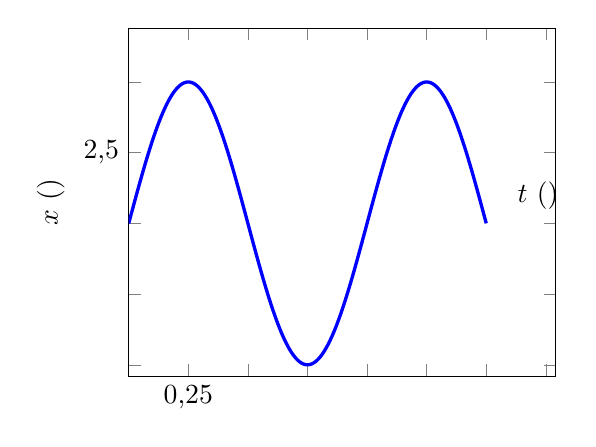
\begin{tikzpicture}
            \def\Xm{5}
            \def\T{1}
            \pgfmathpi\let\pi=\pgfmathresult
            \begin{axis}[
                    xmin=0,xmax=1.79,
                    ymin=-5.4,ymax=6.9,
                    width=7cm,height=6cm,
                    trig format plots=rad,
                    xtick distance=0.25, ytick distance=2.5,
                    xticklabels={,,{0,25}}, yticklabels={,,,,{2,5}},
                    xlabel=$t~(\unit{\second})$, ylabel=$x~(\unit{\cm})$,
	                every axis x label/.append style={
	                	at={(1.03,0.45)},anchor=south east,
	                },
                ]
                \addplot[domain=0:1.5,samples=200,very thick,blue]
                    {\Xm*sin(2*pi/\T*x)};
            \end{axis}
        \end{tikzpicture}
        \caption{}
        \label{fig:xG_de_t}
    \end{subfigure}
    \caption{}
    \label{fig:}
\end{figure}
\begin{enumerate}
    \item Déterminer graphiquement, les valeurs de la période propre $T_{0}$ et
          de l'amplitude $X_{m}$ du mouvement, puis trouver la valeur de $K$ (on
          prendra $\pi^{2}=10$).
    \item Calculer la valeur du travail de la force de rappel exercée sur ($S$)
          entre les instants $(t_{0}=0)$ et $(t_{1}=\frac{T_{0}}{4})$.
    \item En utilisant la conservation de l'énergie mécanique de l'oscillateur,
          déterminer la valeur de la vitesse $v_{0}$ à l'instant ($t_{0}=0$).
\end{enumerate}
